\input{styleDS}
\def\numero{03}
\def\classe{Option info MP1}
\def\sep{\text{sep}}
\def\sur#1#2{${}^{\hbox{#1}}_{\hbox{#2}}$}
\def\sur#1#2{$\begin{matrix}\hbox{#1} \\ \hbox{#2}\end{matrix}$}

\tikzset{fl/.style={ draw, fill = gray,rectangle,minimum size=3mm}}

\camltrue
%-------------------------------------------------------------------------------
%-------------------------------------------------------------------------------
%-------------------------------------------------------------------------------
\begin{document}
%-------------------------------------------------------------------------------
%-------------------------------------------------------------------------------
%-------------------------------------------------------------------------------
\chapter{Arbres binaires}
%-------------------------------------------------------------------------------
%-------------------------------------------------------------------------------
%-------------------------------------------------------------------------------
\section{Arbres d'intervalles, adapté de CCP 2010}
%-------------------------------------------------------------------------------
%-------------------------------------------------------------------------------
%-------------------------------------------------------------------------------
De nombreux algorithmes reposent sur la manipulation d'ensembles d'éléments ordonnés. Lorsque 
ces ensembles contiennent de nombreux éléments adjacents (aucune valeur n'existe entre les deux 
éléments), il est plus performant en terme de temps de calcul et d'occupation mémoire de manipuler 
des intervalles au lieu de valeurs singulières. Cela permet également de manipuler des ensembles 
infinis de réels ou de rationnels sous la forme d`un ensemble fini d'intervalles contenant un 
nombre de valeurs infinies.

Nous nous limiterons à des intervalles fermés de $\R$ dont les bornes 
sont des entiers : $[min; max]$ avec $min \le max$.
%-------------------------------------------------------------------------------
%-------------------------------------------------------------------------------
\subsection{Définitions}
%-------------------------------------------------------------------------------
%-------------------------------------------------------------------------------
\begin{enumerate}
  \item Deux intervalles sont {\bf disjoints} si leur intersection est vide.
  \item La {\bf fusion} de deux intervalles est l'intervalle qui a, comme minimum, le plus petit des
minima des deux intervalles, et comme maximum, le plus grand des maxima des deux intervalles.
Cette opération correspond à l'union des intervalles si ceux-ci ne sont pas disjoints.
\item Un intervalle est représenté par un couple de deux entiers, son minimum en premier et son maximum en second.
\begin{lstlisting}
type intervalle == int * int;;
\end{lstlisting}
\end{enumerate}
%-------------------------------------------------------------------------------
%-------------------------------------------------------------------------------
\begin{Exercise}\it
Écrire une fonction \type{disjoints : intervalle -> intervalle -> bool}

telle que l'appel \type{disjoints i1 i2} renvoie la valeur \type{true} si les intervalles \type{i1} et \type{i2}
sont disjoints et la valeur \type{false} sinon.
\end{Exercise}
%--------------------------------------------------------------------------
\begin{Answer}
Il suffit de vérifier que la borne supérieure d'un intervalle est strictement inférieure à la borne inférieure de l'autre intervalle.
\begin{lstlisting}
let disjoints (min1, max1) (min2, max2) = 
  max1 < min2 || max2 < min2;;
\end{lstlisting}
\end{Answer}
%-------------------------------------------------------------------------------
\smallskip
\type{disjoints (4, 7) (1, 3)} doit renvoyer \type{true}.
%-------------------------------------------------------------------------------
%-------------------------------------------------------------------------------
\begin{Exercise}\it
Écrire une fonction \type{fusion : intervalle -> intervalle -> intervalle}

telle que l'appel \type{fusion i1 i2} renvoie un intervalle correspondant à la
fusion de \type{i1} et \type{i2}.
\end{Exercise}
%--------------------------------------------------------------------------
\begin{Answer}
\begin{lstlisting}
let fusion (min1, max1) (min2, max2) = 
  (min min1 min2), (max max1 max2);;
\end{lstlisting}
\end{Answer}
%-------------------------------------------------------------------------------
%-------------------------------------------------------------------------------

\medskip

Un arbre binaire d'intervalles $a$ est une structure qui peut être :
\begin{itemize}
\item soit vide, notée $\emptyset$,
\item soit une feuille qui contient un intervalle $[min; max]$,
\item soit un nœud qui contient un entier noté $\sep(a)$, un sous-arbre gauche (noté $G(a)$) et un sous-arbre droit (noté $D(a)$) qui sont tous deux des arbres binaires d'intervalles {\bf non vides}.
\item L'union des intervalles d'un arbre $a$ est noté ${\cal E}(a)$.
\end{itemize}

\medskip

Un arbre binaire d'intervalles est représenté par le type CaML :
\begin{lstlisting}
type arbre = Vide
            |Feuille of int * int
            |Noeud of arbre * int * arbre;;
\end{lstlisting}
\medskip
%-------------------------------------------------------------------------------
\begin{minipage}{0.40\textwidth}
  \begin{center}
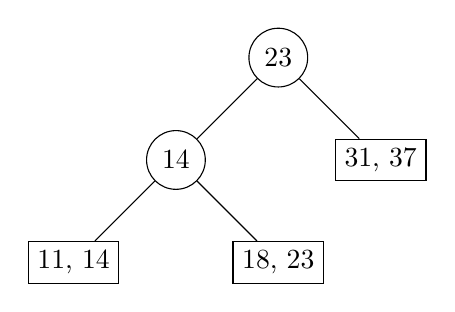
\begin{tikzpicture}[scale  = 0.65]
\tikzstyle{every node}=[draw]
\node(ar)[circle]   at ( 0,  0) {23};
\node(ag)[circle]   at (-2, -2) {14};
\node(ad)           at ( 2, -2) {31, 37};
\node(agg)          at (-4, -4) {11, 14};
\node(agd)          at ( 0, -4) {18, 23};

\draw (ar) -- (ag);
\draw (ar) -- (ad);
\draw (ag) -- (agg);
\draw (ag) -- (agd);

\end{tikzpicture} 

\medskip

Un exemple d'arbre d'intervalle, $a_0$
  \end{center}
\end{minipage}
\begin{minipage}{0.60\textwidth}
\begin{lstlisting}
let a0 = Noeud(Noeud(Feuille(11, 14), 
                     14, 
                     Feuille(18, 23)
                    ), 
               23,
               Feuille(31, 37)
              );;               
\end{lstlisting}
\end{minipage}
%-------------------------------------------------------------------------------
%-------------------------------------------------------------------------------
\begin{Exercise}\it
Écrire une fonction \type{suite : arbre -> intervalle list}

telle que l'appel \type{suite a} renvoie la liste des intervalles des feuilles de \type{a} dans l'ordre obtenu par un parcours (infixe, préfixe ou suffixe) de l'arbre.
\end{Exercise}
%--------------------------------------------------------------------------
\begin{Answer}
\begin{lstlisting}
let rec suite arbre = 
  match arbre with
  |Vide -> []
  |Feuille(a, b) = [(a, b)]
  |Noeud(g, _, d) -> (suite g) @ (suite d);;
\end{lstlisting}
\end{Answer}
%-------------------------------------------------------------------------------
\smallskip
\type{suite a0} doit renvoyer \type{[(11, 14); (18, 23); (31, 37)]}.
%-------------------------------------------------------------------------------
%-------------------------------------------------------------------------------
\medskip

L'{\bf intervalle englobant} d'un arbre d'intervalles, noté $\mathcal{I}(a)$, est le plus petit 
intervalle  qui contient tous les intervalles contenus dans les feuilles de l'arbre.
%-------------------------------------------------------------------------------
%-------------------------------------------------------------------------------
\begin{Exercise}\it
Écrire une fonction \type{englobant : arbre -> intervalle}

telle que l'appel \type{englobant a} renvoie l'intervalle englobant de \type{a} pour \type{a} non vide.
\end{Exercise}
%--------------------------------------------------------------------------
\begin{Answer}
\begin{lstlisting}
let rec englobant a =
  match a with
  |Vide -> failwith "Erreur arbre vide"
  |Feuille(min, max) -> min, max
  |Noeud(g, n, d) -> fusion (englobant fg) (englobant fd);;
\end{lstlisting}
\end{Answer}
%-------------------------------------------------------------------------------
\type{englobant a0} doit renvoyer \type{11, 37}.
%-------------------------------------------------------------------------------
%-------------------------------------------------------------------------------
\medskip

Un arbre d'intervalles {\bf bien formé} est un arbre d'intervalles qui 
respecte les contraintes suivantes : 
\begin{enumerate}
    \item les intervalles contenus dans les feuilles sont disjoints 
    deux à deux,
    \item pour tout nœud $n$, l'intervalle englobant ${\cal G}(n)$, $[min_g; max_g]$, et l'intervalle englobant ${\cal D}(n)$, $[min_d; max_d]$ vérifient $max_g = \sep(n) < min_d$.
\end{enumerate}
$a_0$ est bien formé. Tout arbre vide est bien formé.
%-------------------------------------------------------------------------------
%-------------------------------------------------------------------------------
\begin{Exercise}\it
Écrire une fonction \type{verifie\_bf : arbre -> bool}

telle que l'appel \type{verifie\_bf a} renvoie \type{true} ou \type{false} selon que \type{a} est bien formé ou non.

On privilégiera  un algorithme qui ne parcourt qu'une seule fois l'arbre.
\end{Exercise}
%--------------------------------------------------------------------------
\begin{Answer}
On écrit une fonction auxiliaire récursive qui retourne l'intervalle englobant en même temps que la réponse booléenne.
\begin{lstlisting}
let verifie a =
  let rec aux a = 
    match a with
    |Vide -> true, 0, 0
    |Feuille(min, max) -> true, min, max
    |Noeud(g, n, d) -> let rep1, min1, max1 = aux g in
                       let rep2, min2, max2 = aux d in
                       let rep = rep1 && rep2 && (max1 = k) && (k < min2) in
                       rep, min1, max2 in
  let rep, _, _ = aux a in rep;;
\end{lstlisting}
\end{Answer}
%-------------------------------------------------------------------------------
%-------------------------------------------------------------------------------
\begin{Exercise}\it
Écrire une fonction \type{appartient : int -> arbre -> bool}

telle que l'appel \type{appartient k a} renvoie \type{true} ou \type{false} selon que \type{k} appartient ou non à l'un des intervalles de \type{a} qu'on suppose bien formé.

On attend une complexité proportionnelle à la hauteur de l'arbre.
\end{Exercise}
%--------------------------------------------------------------------------
\begin{Answer}
\begin{lstlisting}
let rec appartient k a =
  match a with
  |Vide -> false
  |Feuille(min, max) -> (min <= k) && (k <= max)
  |Noeud(g, n, d) when n < k -> appartient k d
  |Noeud(g, n, d) -> appartient k g;;
\end{lstlisting}
\end{Answer}
%-------------------------------------------------------------------------------
%-------------------------------------------------------------------------------
Les entiers de ${\cal E}(a)$ sont les entiers $k$ tels que \type{appartient k a} renvoie \type{true}.
%-------------------------------------------------------------------------------
%-------------------------------------------------------------------------------
\begin{Exercise}\it
Écrire une fonction \type{ajoute\_simple : intervalle -> arbre -> bool}

telle que l'appel \type{ajoute\_simple (min, max) a} renvoie un arbre d'intervalle bien formé contenant les intervalles de \type{a} et l'intervalle \type{(min, max)}.

On suppose que \type{a} est bien formé et que \type{(min, max)} est disjoint de tous les intervalles de \type{a}.

On attend une complexité proportionnelle à la hauteur de l'arbre.
\end{Exercise}
%--------------------------------------------------------------------------
\begin{Answer}
Dans le cas simple de l'énoncé, comme la valeur d'un nœud appartient à l'un des intervalles du fils gauche, on n'aura jamais cette valeur dans l'intervalle à ajouter. On ne pourra donc rencontrer que le cas $n< min$ ou $max < n$. De même quand on arrive à une feuille, comme les intervalles sont disjoints il y en aura un à droite de l'autre.
\begin{lstlisting}
let rec ajouter (min, max) a =
  match a with
  |Vide -> Feuille( min, max)
  |Feuille(min1, max1) when max1 < min -> 
          Noeud(a, max1, Feuille(min, max))
  |Feuille(min1, max1) -> Noeud( Feuille(min, max), max, a)
  |Noeud(g, n, d) when n < min -> Noeud(g, n, ajouter (min, max) d)
  |Noeud(g, n, d) -> Noeud(ajouter (min, max) g, n, d);;
  
\end{lstlisting}
\end{Answer}
%-------------------------------------------------------------------------------
%-------------------------------------------------------------------------------
% \begin{Exercise}\it
% Écrire une fonction \type{decoupe : intervalle -> arbre -> arbre * arbre * arbre}
%
% telle que l'appel \type{decoupe (min, max) a} avec \type{a} bien formé renvoie un triplet composé
%
% \begin{itemize}
%     \item d'un arbre bien formé contenant les intervalles strictement inférieurs à la valeur \type{min}, 
%     \item d'un arbre bien formé contenant les intervalles dont l'intersection avec \type{(min, max)} est non vide
%     \item d'un arbre bien formé contenant les intervalles strictement supérieurs à la valeur \type{max}.
% \end{itemize}
% \end{Exercise}
% %--------------------------------------------------------------------------
% \begin{Answer}
% \begin{lstlisting}
% \end{lstlisting}
% \end{Answer}
% %-------------------------------------------------------------------------------
% %-------------------------------------------------------------------------------
% \begin{Exercise}\it
% Écrire une fonction \type{ajoute : intervalle -> arbre -> bool}
%
% telle que l'appel \type{ajoute i a} renvoie un arbre d'intervalle bien formé contenant 
% \begin{enumerate}
%   \item les intervalles de \type{a} qui sont disjoints de \type{i} et 
%   \item le résultat de la fusion de \type{i} et des intervalles de \type{a} qui ne sont pas disjoints de \type{i}. 
% \end{enumerate}
%
% On suppose que \type{a} est bien formé mais on ne suppose plus que \type{i} est disjoint des intervalles de \type{a}.
% \end{Exercise}
% %--------------------------------------------------------------------------
% \begin{Answer}
% \begin{lstlisting}
% \end{lstlisting}
% \end{Answer}
% %-------------------------------------------------------------------------------
%-------------------------------------------------------------------------------
%-------------------------------------------------------------------------------
\section{Arbres de Huffman, Mines 2006}
%-------------------------------------------------------------------------------
%-------------------------------------------------------------------------------
%-------------------------------------------------------------------------------

{\it Le problème est consacré à l’algorithme de Huffman qui permet de coder un texte caractère par
caractère à l’aide d’une chaîne binaire en minimisant la longueur totale de la chaîne obtenue ; cet algorithme
permet de faire de la compression de données. Les parties 1 et 2 du problème sont des parties préparatoires, le
codage d’un texte sera abordé dans la troisième partie.}

\medskip


Dans tout le problème, on utilise des arbres binaires. 

Pour un arbre, les termes de nœud et de sommet sont
synonymes ; c’est le terme de nœud qui est retenu dans ce problème. Un nœud qui n’a pas de fils est appelé
{\bf feuille} alors qu’un nœud qui a au moins un fils est appelé un {\bf nœud interne}.

Chaque nœud $n$ des arbres binaires de ce problème contient, outre les indications concernant ses éventuels
fils gauche et droit (voir plus bas), un caractère appelé {\bf lettre du nœud} et noté {\it lettre(n)} et un entier strictement positif appelé {\bf poids du nœud} et noté {\it poids(n)}. 

Ces arbres binaires sont appelés {\bf H\_arbres}.

Une {\bf forêt} est dans ce sujet une collection de H\_arbres.

Une forêt est représentée en mémoire par :
\begin{itemize}
  \item le nombre de H\_arbres de la forêt, noté {\it nb\_arbres},
  \item le nombre total de nœuds, noté {\it nb\_nœuds},
  \item un tableau de nœuds appelé {\it table}. Dans tout le problème, ce tableau est supposé
suffisamment grand pour contenir les nœuds de tous les H\_arbres de la forêt considérée, les nœuds sont
rangés dans le tableau entre les indices 0 et {\it nb\_nœuds - 1}
\end{itemize}
ATTENTION : les nœuds qui sont les racines des H\_arbres de la forêt se trouvent nécessairement au début du tableau {\it table}, c’est-à-dire entre les indices 0 et {\it nb\_arbres - 1}. 

Pour un nœud donné, les fils gauche et droit sont indiqués par leurs indices dans le tableau table des nœuds ; lorsqu’un fils gauche ou droit n’existe pas, cela est indiqué par une valeur d’indice égale à $-1$. Le fils gauche d’un nœud $n$ sera noté {\it fg(n)} et le fils droit sera noté {\it fd(n)}.
%-------------------------------------------------------------------------------
\begin{figure}[ht]
  \begin{center}
\begin{tikzpicture}
\tikzstyle{every node}=[circle,draw]
\node(n0) at (-0.5, 0) {\sur{'g'}2};%{'g', 2};
\node(n1) at (4, 0) {\sur{'a'} 7};
\node(n2) at (8, 0) {\sur{'b'} 4};
\node(n3) at (5.5, -1.5) {\sur{'e'} 3};
\node(n4) at (2.5, -1.5) {\sur{'f'} 5};
\node(n5) at (4.5, -3) {\sur{'c'} 4};
\node(n6) at (0.5, -1.5) {\sur{'d'} 5};
\draw (n0) -- (n6);
\draw (n1) -- (n4);
\draw (n1) -- (n3);
\draw (n3) -- (n5);
\end{tikzpicture} 
    \caption{Un exemple introductif, noté {\it F\_ex}}
  \end{center}
\end{figure}
%-------------------------------------------------------------------------------

\medskip
Pour la forêt  {\it F\_ex}, on a : {\it nb\_arbres} = 3, {\it nb\_nœuds} = 7 ; une table qui peut la représenter est
%-------------------------------------------------------------------------------
  \begin{center}
    \begin{tabular}{r|ccccccc}
     Indice du nœud  & 0&1&2&3&4&5&6\\
     \hline
     Lettre  & 'g'&'a'&'b'&'e'&'f'&'c'&'d'\\
     Poids & 2&7&4&3&5&4&5\\
     Fils gauche &-1&4&-1&5&-1&-1&-1\\
     Fils droit &6&3&-1&-1&-1&-1&-1\\
    \end{tabular}
  \end{center}
%-------------------------------------------------------------------------------
  Dans cette table, on voit que le nœud d’indice 3 contient la lettre ‘e’ et le poids 3, que son fils gauche se
trouve à l’indice 5 de la table et qu’il n’a pas de fils droit.

\newpage
On définit les types suivants
%-------------------------------------------------------------------------------
\begin{lstlisting}
type noeud = {lettre : char;  poids : int; 
                  fg : int;      fd : int};;

type foret= {mutable nb_arbres : int; 
             mutable nb_noeuds : int; 
                         table : noeud array};;
\end{lstlisting}
%-------------------------------------------------------------------------------
On définit un nœud vide comme valeur par défaut dans la définition d'un tableau de nœuds :
%-------------------------------------------------------------------------------
\begin{lstlisting}
let noeud_vide = {lettre='\000'; poids=0; fg=(-1); fd=(-1)};;
\end{lstlisting}
%-------------------------------------------------------------------------------
La forêt {\it F\_ex} de l’exemple introductif peut être définie par :
%-------------------------------------------------------------------------------
\begin{lstlisting}
let f_ex =
  let table_ex = Array.make 100 noeud_vide in
  table_ex.(0) <- {lettre='g'; poids=2; fg=(-1); fd=6};
  table_ex.(1) <- {lettre='a'; poids=7; fg=4; fd=3};
  table_ex.(2) <- {lettre='b'; poids=4; fg=(-1); fd=(-1)};
  table_ex.(3) <- {lettre='e'; poids=3; fg=5; fd=(-1)};
  table_ex.(4) <- {lettre='f'; poids=5; fg=(-1); fd=(-1)};
  table_ex.(5) <- {lettre='c'; poids=4; fg=(-1); fd=(-1)};
  table_ex.(6) <- {lettre='d'; poids=5; fg=(-1); fd=(-1)};
  {nb_arbres = 3; nb_noeuds = 7; table = table_ex};;
\end{lstlisting}

%-------------------------------------------------------------------------------

On supposera que la table est assez grande pour pouvoir contenir les nœuds qui seront ajoutés.

\medskip

{\bf Remarques sur la syntaxe} 

\begin{enumerate}
  \item Le poids du nœud d'indice $k$ dans un arbre \type{a} est lu par \type{a.table.(0).poids},

\item La modification d’un champ mutable se fait à l’aide du signe \type{<-} ; on pourra, par exemple, 
écrire \type{a.nb\_arbres <- 2} pour indiquer que la forêt \type{a} contient dorénavant deux H\_arbres.
\end{enumerate}

%-------------------------------------------------------------------------------
%-------------------------------------------------------------------------------
\subsection{Fonctions de base pour l’algorithme de Huffman}
%-------------------------------------------------------------------------------
%-------------------------------------------------------------------------------
On considère une forêt contenant {\it nb\_nœuds} nœuds et un entier $k$ vérifiant $1 \le k \le \text{\it nb\_nœuds}$ ; il
s’agit d’écrire une fonction déterminant l’indice du nœud dont le poids est le plus petit parmi les $k$
premiers nœuds de la table de la forêt, c’est-à-dire parmi les nœuds qui se trouvent entre les indices 0 et
$k - 1$ de cette table. S’il y a plusieurs nœuds de plus petit poids dans l’intervalle indiqué, la fonction
renverra le plus petit indice de ceux-ci.
%-------------------------------------------------------------------------------
%-------------------------------------------------------------------------------
\begin{Exercise}[label = ques:min]\it 
Écrire une fonction \type{indice\_du\_min} telle que si \type{f} est une valeur de type \type{foret} et \type{k} une valeur entière strictement positive ne dépassant pas \type{f.nb\_noeuds}, alors \type{indice\_du\_min f k} renvoie l’indice recherché.
\end{Exercise}
%--------------------------------------------------------------------------
\begin{Answer}
\begin{lstlisting}
let indice_du_min foret k =
  let mini = ref foret.table.(0).poids in
  let ind_mini = ref 0 in
  for i = 1 to k-1 do
    if foret.table.(i).poids < !mini
    then (ind_mini := i;
          mini := foret.table.(i).poids) done;
  !ind_mini;;
\end{lstlisting}
\end{Answer}
%-------------------------------------------------------------------------------
%-------------------------------------------------------------------------------
\medskip
On considère une forêt $F$ constitué d’au moins deux H\_arbres. Il s’agit de faire en sorte que, dans
la table de $F$, les deux racines de plus petits poids soient les deux dernières racines dans la partie de la
table consacrée aux racines de la forêt. Autrement dit, il s’agit d’examiner les racines de $F$ (c’est-à-dire
les nœuds qui se trouvent entre les indices 0 et $\text{\it nb\_arbres} - 1$ de la table) pour mettre, par des échanges,
les deux racines de plus petits poids aux indices $\text{\it nb\_arbres} - 2$ et $\text{\it nb\_arbres} - 1$ ; plus précisément, on mettra la racine de plus petit poids à l’indice $\text{\it nb\_arbres} - 1$ et la racine d’avant-dernier plus petit poids à l’indice $\text{\it nb\_arbres} - 2$. 

\newpage

Par exemple, après ce traitement, la table décrivant {\it F\_ex} devient :
%-------------------------------------------------------------------------------
  \begin{center}
    \begin{tabular}{r|ccccccc}
     Indice du nœud  & 0&1&2&3&4&5&6\\
     \hline
     Lettre  & 'a'&'b'&'g'&'e'&'f'&'c'&'d'\\
     Poids & 7&4&2&3&5&4&5\\
     Fils gauche &4&-1&-1&5&-1&-1&-1\\
     Fils droit &3&-1&6&-1&-1&-1&-1\\
    \end{tabular}
  \end{center}
%-------------------------------------------------------------------------------
S’il y a des égalités entre les poids qui conduisent à plusieurs couples possibles de racines de plus petits
poids, on choisira alors les deux racines de plus petits indices. On utilisera la fonction définie dans la
question \ref{ques:min}.
%-------------------------------------------------------------------------------
%-------------------------------------------------------------------------------
\begin{Exercise}[label = ques:2min]\it
Écrire une fonction \type{deux\_plus\_petits} telle que si \type{f} est une valeur de type \type{foret}
vérifiant \type{f. nb\_arbres >= 2}, alors \type{deux\_plus\_petits f} transforme le champ \type{table} de \type{f} de
façon à obtenir l’ordre cherché.
\end{Exercise}
%--------------------------------------------------------------------------
\begin{Answer}
Je note $k$ la valeur de {\it nb\_arbres}. On opère en deux temps, 
\begin{enumerate}
  \item on cherche le minimum parmi les $n$ premiers arbres,
  \item on le place en position $n$,
  \item on cherche le minimum parmi les $n-1$ premiers arbres,
  \item on le place en position $n-1$.  
\end{enumerate}

On commence par une fonction d'échange :

\begin{lstlisting}
let echange i j foret = 
  let noeud = foret.table.(i) in
  foret.table.(i) <- foret.table.(j);
  foret.table.(j) <- noeud;;
\end{lstlisting}

On peut alors traduire l'algorithme.

\begin{lstlisting}
let deux_plus_petits foret = 
  let k = foret.nb_arbres in
  if k >= 2
  then begin let i = indice_du_min foret k     
             in echange i (k-1) foret;
             let j = indice_du_min foret (k-1) 
             in echange j (k-2) foret end;;
\end{lstlisting}

\newpage
\end{Answer}
%-------------------------------------------------------------------------------
%-------------------------------------------------------------------------------
\medskip

On considère une forêt $F$ possédant au moins deux H\_arbres. On définit une transformation de $F$
nommée assemblage de $F$. Soient $r_1$ et $r_2$ deux racines de plus petits poids ; on suppose que le poids de $r_1$
est inférieur ou égal à celui de $r_2$ . L’assemblage de $F$ consiste à ajouter à $F$ un nœud dont :
\begin{itemize}
  \item le poids est la somme des poids des nœuds $r_1$ et $r_2$,
  \item le fils gauche est $r_1$,
  \item le fils droit est $r_2$.
\end{itemize}
Le nœud ajouté est donc la racine d’un H\_arbre de la forêt obtenue par l’assemblage et le nombre total de H\_arbres de la forêt a diminué de 1.

La lettre contenue par ce nouveau nœud n’a pas d’importance et n’est pas spécifiée. On ne cherche pas à
ce que, après assemblage, les racines des H\_arbres respectent l’ordre de la question \ref{ques:2min}.

Si on applique cette transformation à la forêt {\it F\_ex}, celle-ci devient la forêt ci-dessous, dans laquelle on
n’a pas précisé de valeur pour la lettre du nœud ajouté :
%-------------------------------------------------------------------------------
\begin{center}
\begin{tikzpicture}
\tikzstyle{every node}=[circle,draw]
\node(n0) at (8, -1.5) {\sur{'g'} 2};
\node(n1) at (4, 0) {\sur{'a'} 7};
\node(n2) at (11, -1.5) {\sur{'b'} 4};
\node(n3) at (5.5, -1.5) {\sur{'e'} 3};
\node(n4) at (2.5, -1.5) {\sur{'f'} 5};
\node(n5) at (4.5, -3) {\sur{'c'} 4};
\node(n6) at (9, -3) {\sur{'d'} 5};
\node(n7) at (9.5, 0) {\_, 6};
\draw (n0) -- (n6);
\draw (n1) -- (n4);
\draw (n1) -- (n3);
\draw (n3) -- (n5);
\draw (n7) -- (n0);
\draw (n7) -- (n2);
\end{tikzpicture} 
\end{center}
%-------------------------------------------------------------------------------
Pour cette forêt, on a \text{\it nb\_arbres} = 2, {\it nb\_nœuds} = 8 et la table peut être
%-------------------------------------------------------------------------------
  \begin{center}
    \begin{tabular}{r|cccccccc}
     Indice du nœud  & 0&1&2&3&4&5&6&7\\
     \hline
     Lettre  & 'a'&\_&'g'&'e'&'f'&'c'&'d'&'b'\\
     Poids & 7&6&2&3&5&4&5&4\\
     Fils gauche &4&2&-1&5&-1&-1&-1&-1\\
     Fils droit &3&7&6&-1&-1&-1&-1&-1\\
    \end{tabular}
  \end{center}
%-------------------------------------------------------------------------------
%-------------------------------------------------------------------------------
\begin{Exercise}\it
Écrire en une fonction assemblage telle que, si \type{f} est une valeur de type \type{foret}
vérifiant 

\type{f.nb\_arbres >= 2}, alors \type{assemblage f} transforme \type{f} selon les indications fournies ci- dessus. 

On utilisera la fonction \type{deux\_plus\_petits} définie dans la question précédente.
\end{Exercise}
%--------------------------------------------------------------------------
\begin{Answer}
Le nouvel arbre devra être à la $k-1$-ième position, celle occupée par l'avant-dernière racine.

On note $k$ le nombre d'arbres et $n$ le nombre de nœuds :

\begin{itemize}
\item on place les deux arbres de poids minimal à la fin des arbres (question ci-dessus)
\item on copie le nœud d'indice $k-2$ (l'avant dernier arbre) à la position $n$,
\item on place à la position $k-2$ un nouveau nœud, sa somme est la somme des deux poids, son fils gauche a l'indice $k-1$ et son fils droit a l'indice $n$,
\item on augmente $n$ de 1, on ajoute un nouvel nœud
\item on diminue $k$ de 1, le nouveau nœud remplace deux arbres.
\end{itemize}

\begin{lstlisting}
let assemblage f = 
  let n = f.nb_noeuds in
  let k = f.nb_arbres in
  if k >= 2
  then begin
    deux_plus_petits f;
    f.table.(n) <- f.table.(k-2);
    f.table.(k-2) <- 
      {lettre = `\000`; fg = (k-1); fd = n;
       poids = f.table.(n).poids + f.table.(k-1).poids};
    f.nb_noeuds <- (n+1);
    f.nb_arbres <- (k-1) 
  end;;
\end{lstlisting}
\end{Answer}
%-------------------------------------------------------------------------------
\newpage
%-------------------------------------------------------------------------------
\subsection{Propriétés pour l’algorithme de Huffman}
%-------------------------------------------------------------------------------
%-------------------------------------------------------------------------------
Remarque : dans les illustrations de cette partie, lorsqu’un champ n’est pas précisé dans un nœud, cela
signifie que sa valeur n’intervient pas.

La hauteur d’un nœud $n$ d’un arbre, notée $h(n)$, est définie de la façon suivante :
\begin{itemize}
  \item la hauteur de la racine vaut 0,
  \item la hauteur d’un nœud autre que la racine vaut un de plus que la hauteur de son père.
\end{itemize}

On dit, dans un arbre, qu’un nœud $n$ est de {\bf hauteur maximum} s’il n’existe pas de nœud de hauteur
strictement plus grande que $h(n)$ dans cet arbre ; un nœud de hauteur maximum est nécessairement une feuille.

Deux feuilles d’un arbre sont dites {\bf sœurs} si elles ont le même nœud pour père.

Étant donné un H\_arbre $A$, on appelle {\bf évaluation} de $A$ la quantité $\displaystyle e(A) = \sum_{f \text{ feuille de }A}
h(f).\text{\it poids}(f)$.

Pour l'arbre {\it A\_ex} ci-dessous, on a $e(\text{\it A\_ex}) = 1\times 5 + 3 \times 4 + 3 \times 7 = 38$.
%-------------------------------------------------------------------------------
%-------------------------------------------------------------------------------
\begin{Exercise}\it
Écrire une fonction \type{eval} telle que, si \type{f} est une valeur de type \type{foret}, alors \type{eval f} calcule la somme des évaluations des arbres qui composent la forêt..
\end{Exercise}
%--------------------------------------------------------------------------
\begin{Answer}

On calcule l'évaluation d'un arbre en calculant la somme des évaluations de ses fils. On a besoin d'envoyer un paramètre hauteur pour calculer l'évaluation des feuilles.
\begin{lstlisting}
let eval f =
  let rec eval_arbre arbre haut =
    match arbre.fg, arbre.fd with 
    |-1, -1 -> arbre.poids*h
    |-1, k -> eval_arbre f.(k) (haut + 1)
    |k, -1 -> eval_arbre f.(k) (haut + 1)
    |k, l -> eval_arbre f.(k) (haut + 1) + eval_arbre f.(l) (haut + 1)
  in let e = ref 0 in
     for i = 0 to (nb_arbres -1) 
       do e := !e +eval_arbre f.(i) 0 done;
     !e;;
\end{lstlisting}
\end{Answer}
%-------------------------------------------------------------------------------
%-------------------------------------------------------------------------------
\medskip

On rappelle que les poids des nœuds sont des entiers strictement positifs.

On dit que deux H\_arbres ont mêmes feuilles s’ils ont le même nombre de feuilles et que les contenus des
feuilles de l’un sont les mêmes que les contenus des feuilles de l’autre. 

On dira par exemple que les deux
H\_arbres {\it A\_ex} et {\it A'\_ex} ci-dessous ont mêmes feuilles.
%-------------------------------------------------------------------------------
\begin{figure}[ht]
  \begin{center}
\begin{tikzpicture}[scale  = 0.65]
\tikzstyle{every node}=[circle,draw]
\node(ar)   at ( 0,   0) {\sur{-}{-}};
\node(ag)   at (-2,  -2) {\sur{'c'}  5};
\node(ad)   at ( 2,  -2) {\sur{-}{-}};
\node(adg)  at ( 0,  -4) {\sur{-}{-}};
\node(adgg) at (-2,  -6) {\sur{'a'}  4};
\node(adgd) at ( 2,  -6) {\sur{'b'}  7};
\node(br)   at (11,   0) {\sur{-}{-}};
\node(bg)   at ( 9,  -2) {\sur{-}{-}};
\node(bd)   at (13,  -2) {\sur{-}{-}};
\node(bgg)  at ( 7,  -4) {\sur{-}{-}};
\node(bgd)  at (11,  -4) {\sur{'a'}  4};
\node(bdd)  at (15,  -4) {\sur{'b'}  7};
\node(bggg) at ( 5,  -6) {\sur{'c'}  5};

\draw (ar) -- (ag);
\draw (ar) -- (ad);
\draw (ad) -- (adg);
\draw (adg) -- (adgg);
\draw (adg) -- (adgd);
\draw (br) -- (bg);
\draw (br) -- (bd);
\draw (bg) -- (bgg);
\draw (bg) -- (bgd);
\draw (bd) -- (bdd);
\draw (bgg) -- (bggg);
\end{tikzpicture} 
    \caption{Deux arbres, {\it A\_ex} et {\it A'\_ex}}
  \end{center}
\end{figure}
%-------------------------------------------------------------------------------
%-------------------------------------------------------------------------------
\begin{Exercise}\it
Montrer que, si un H\_arbre $A$ est optimal, alors tout nœud interne de $A$ admet deux fils. Après
avoir montré ce résultat, transformer le H\_arbre {\it A\_ex} en un H\_arbre {\it B\_ex} de mêmes feuilles que {\it A\_ex} et d’évaluation inférieure en s’appuyant sur l’argument de la preuve ; on indiquera pour cet exemple le gain
d’évaluation obtenu.
\end{Exercise}
%--------------------------------------------------------------------------
\begin{Answer}
Si $a$ est un arbre dont un nœud interne $n$ n'a un seul fils, par exemple le fils gauche $g$, on remplace le nœud $n$ par son fils gauche $g$. L'arbre obtenu, noté $a'$, a les mêmes feuilles  mais les feuilles qui figuraient dans $g$ ont maintenant une hauteur diminuée de 1. Ainsi, si  $p$ est la somme des poids des feuilles dans $g$, on a $e(a') = e(a) -p$.

Les poids sont strictement positifs et tout nœud interne contient au moins une feuille donc $p>0$.
On obtient donc $e(a') < e(a)$ et $a'$ contient les mêmes feuilles que $a$ donc $a$ n'est pas optimal.

Par contraposition dans un arbre optimal tout nœud interne a exactement deux fils.

Cette procédure appliquée à $A\_{ex}$ donne l'arbre $B\_{ex}$ suivant.

\begin{center}
\begin{tikzpicture}[scale  = 0.65]
\tikzstyle{every node}=[circle,draw]
\node(ar)   at ( 0,   0) {\sur{-}{-}};
\node(ag)   at (-2,  -2) {\sur{'c'}  5};
\node(ad)   at ( 2,  -2) {\sur{-}{-}};
\node(adg)  at ( 0,  -4) {\sur{'a'}  4};
\node(add)  at ( 4,  -4) {\sur{'b'}  7};

\draw (ar) -- (ag);
\draw (ar) -- (ad);
\draw (ad) -- (adg);
\draw (ad) -- (add);
\end{tikzpicture} 
\end{center}

L'évaluation de $B\_{ex}$ vaut $1.5 + 2.4 + 2.7 = 27 = 38-11$.
\end{Answer}
%-------------------------------------------------------------------------------
%-------------------------------------------------------------------------------
\begin{Exercise}\it
Soient $f_1$ et $f_2$ deux feuilles d’un H\_arbre $A$ optimal vérifiant la relation $h(f_1) > h(f_2)$ ; montrer
qu’alors on a $\text{\it poids}(f_1) \le \text{\it poids}(f_2)$. Après avoir montré ce résultat, transformer le H\_arbre {\it B\_ex} en un H\_arbre {\it C\_ex} de mêmes feuilles et d’évaluation inférieure à celle de {\it C\_ex} ; on indiquera le gain d’évaluation obtenu.
\end{Exercise}
%--------------------------------------------------------------------------
\begin{Answer}
On considère deux feuilles, $f_1$ et $f_2$, d'un arbre optimal $a$ telles que $h(f_1) = h_1 > h_2 = h(f_2)$.

Si on avait $\hbox{poids}(f_1) = p_1 > p_2 = \hbox{poids}(f_2)$ on pourrait construire un arbre $a'$ égal à $a$ à l'exception de l'échange des feuilles $f_1$ et $f_2$. 

L'évaluation due à la feuille $f_1$ passerait de $h_1p_1$ à $h_2p_1$ et celle de $f_1$ passerait de $h_2p_2$ à $h_1p_2$ d'où $e(a') =e(a) -h_1p_1 + h_2p_1 - h_2p_2 + h_1p_2=e(a)+(p_1-p_2)(h_2-h_1) < e(a)$ ce qui est impossible en raison du caractère optimal de $a$.
On doit donc avoir $\hbox{poids}(f_1) \le  \hbox{poids}(f_2)$.

\medskip

On peut appliquer cette méthode à $B\_{ex}$ pour obtenir $C\_{ex}$ d'évaluation 25 en échangeant les feuilles 'c' et 'b'.
\begin{center}
\begin{tikzpicture}[scale  = 0.65]
\tikzstyle{every node}=[circle,draw]
\node(ar)   at ( 0,   0) {\sur{-}{-}};
\node(ag)   at (-2,  -2) {\sur{'b'}  7};
\node(ad)   at ( 2,  -2) {\sur{-}{-}};
\node(adg)  at ( 0,  -4) {\sur{'a'}  4};
\node(add)  at ( 4,  -4) {\sur{'c'}  5};

\draw (ar) -- (ag);
\draw (ar) -- (ad);
\draw (ad) -- (adg);
\draw (ad) -- (add);
\end{tikzpicture} 
\end{center}

\end{Answer}
%-------------------------------------------------------------------------------
%-------------------------------------------------------------------------------
\begin{Exercise}[label=ques:2soeurs]\it
On considère un H\_arbre $A$ et deux feuilles $f_1$ et $f_2$ de $A$ de plus petits poids. Montrer qu’il existe
un H\_arbre optimal de mêmes feuilles que $A$ dans lequel $f_1$ et $f_2$ sont de hauteur maximum et sont sœurs.
\end{Exercise}
%--------------------------------------------------------------------------
\begin{Answer}
\begin{itemize}
\item on suppose que $f_1$ est de poids minimal. Si $f_1$ n'est pas à la hauteur maximale, pour toute feuille $f$ de hauteur maximale on a $h(f) > h(f_1)$ donc, d'après la question précédente, $\text{\it poids}(f) \le \text{\it poids}(f_1)$. On en déduit , en raison de la minimalité que $\text{\it poids}(f) = \text{\it poids}(f_1)$.

On peut alors échanger les feuille $f$ et $f_1$ sans changer l'évaluation.

{\bf Il existe un arbre optimal $A_1$, de mêmes feuilles que $A$, dans lequel $f_1$ est de hauteur maximale.}
\item On a vu que, dans un arbre optimal, tout nœud interne admet deux fils. 

Une feuille de hauteur maximale admet un père qui est un nœud interne donc admet donc deux fils. Le second fils est aussi une feuille car, sinon, il y aurait des feuille à une hauteur supérieure, ce qui est impossible.

On considère la feuille $f'$, sœur de $f_1$ dans $A_1$.

On a $\text{\it poids}(f') \ge \text{\it poids}(f_2)$ car $f_1$ a le deuxième poids minimal et $f'\ne f_1$.

\item Si $\text{\it poids}(f') =  \text{\it poids}(f_2)$ alors on peut échanger $f'$ et $f_2$ sans changer l'évaluation : on obtient un arbre optimal de mêmes feuilles que $A_1$ donc de même feuilles que $A$ dans lequel $f_1$ et $f_2$ sont de hauteur maximum et sœurs.

\item Si $\text{\it poids}(f') >  \text{\it poids}(f_2)$ $f_2$ est aussi à la hauteur maximale car sinon on aurait 
$h(f') > h(f_2)$ et la question précédente prouverait qu'alors on a $\text{\it poids}(f') \le \text{\it poids}(f_2)$, ce qui est exclu. $f'$ et $f_2$ sont donc à la hauteur maximale et on peut échanger $f'$ et $f_2$ sans changer l'évaluation: on obtient un arbre optimal de mêmes feuilles que $A_1$ donc de même feuilles que $A$ dans lequel $f_1$ et $f_2$ sont de hauteur maximum et sœurs.
\end{itemize}
\end{Answer}
%-------------------------------------------------------------------------------
%-------------------------------------------------------------------------------
\medskip

On considère un H\_arbre $A$ et deux feuilles $f_1$ et $f_2$ qui sont sœurs dans $A$ ; on note $p_1$ et $p_2$ les poids respectifs de ces feuilles. On note $n$ le père (commun) de $f_1$ et $f_2$ et on considère la transformation suivante :
\begin{itemize}
  \item {\it poids(n)} devient égal à $p_1+p_2$,
  \item  on supprime $f_1$ et $f_2$, $n$ devient donc une feuille.
\end{itemize}
Le champ {\it lettre(n)} n’a pas d’importance et n’est donc pas spécifié.

On note $B$ le H\_arbre ainsi obtenu.

On dit qu’on a obtenu $B$ en simplifiant $A$ {\bf par coupe} de $f_1$ et $f_2$ .
%-------------------------------------------------------------------------------
%-------------------------------------------------------------------------------
\begin{Exercise}\it
Établir une relation entre $e(A)$, $e(B)$, $p_1$ et $p_2$ .
\end{Exercise}
%--------------------------------------------------------------------------
\begin{Answer}
 Avec les notations de l'énoncé on a $h(f_1)=h(f_2)=h(n)+1$ donc

$e(B)=e(A)-p_1h(f_1)-p_2h(f_2)+(p_1+p_2)h(n)=e(A)-(p_1+p_2)$
\end{Answer}
%-------------------------------------------------------------------------------
%-------------------------------------------------------------------------------
\begin{Exercise}[label=ques:coupe_opt]\it
On considère maintenant un H\_arbre $A$ et deux feuilles $f_1$ et $f_2$ qui sont sœurs dans $A$ et de plus
petits poids. On simplifie $A$ par coupe de $f_1$ et $f_2$ et on obtient ainsi un H\_arbre $B$. Montrer que $A$ est
optimal si et seulement si $B$ est optimal.
\end{Exercise}
%--------------------------------------------------------------------------
\begin{Answer}On garde les notations de la question précédente.

\begin{itemize}
\item On suppose que $A$ est optimal.
 
Soit $B'$ un arbre de mêmes feuilles que $B$. On peut remplacer la feuille de poids $p_1+p_2$ par un nœud interne qui admet deux fils dont les feuilles ont les poids $p_1$ et $p_2$ par la construction inverse de celle ci-dessus. On obtint un arbre $A'$ qui a les mêmes feuilles que $A$ donc $e(A') \ge e(A)$ car $A$ est optimal. De plus, comme ci-dessus, $e(B') = e(A')-(p_1+p_2)$

On a donc $e(B') = e(A')-(p_1+p_2) \ge e(A)-(p_1+p_2) = e(B)$ pour tout arbre $B'$ de même feuilles que $B$ donc $B$ est optimal.

\item On suppose que $B$ est optimal.

On choisit un arbre optimal $A'$ de même feuilles que $A$. 

D'après la question \ref{ques:2soeurs} on peut supposer que $f_1$ et $f_2$ sont sœurs dans $A'$.
En regroupant $f_1$ et $f_2$ on peut associer à $A'$ un arbre $B'$ qui admet les mêmes feuilles que $B$.

On a $e(A') \le e(A)$ car $A"$ est optimal et, en raison de l'optimalité de $B$,

$e(A')= e(B') + (p_1+p_2) \ge e(B) + (p_1+p_2) =e(A)$ donc $e(A')=e(A)$.

Ainsi $A$ est optimal.
\end{itemize}
\end{Answer}
%-------------------------------------------------------------------------------
%-------------------------------------------------------------------------------
\subsection{Algorithme de Huffman}
%-------------------------------------------------------------------------------
%-------------------------------------------------------------------------------
On appelle {\bf chaîne binaire} une suite composée de 0 et de 1.

On considère dans toute cette partie un texte, c'est-à-dire une chaîne de caractères, $T$.

On souhaite coder ce texte avec une chaîne binaire. Pour cela, on décide d’associer une chaîne binaire à chaque
caractère : son {\bf mot de code} ; l’ensemble des mots de code est le {\bf codage}. On peut alors coder le texte caractère par caractère en mettant bout à bout successivement les mots de code de tous les caractères de $T$ ; on obtient alors le texte codé qui sera noté $C(T)$.

L’objectif est de choisir les mots de code pour que le décodage du texte soit possible et que la chaîne binaire
$C(T)$ soit la plus courte possible.

Dans les exemples on utilisera des textes écrits uniquement avec les 6 lettres 'a', 'b', 'c', 'd', 'e' et 'f' dont on dira qu'elles forment un {\bf alphabet réduit}.
%-------------------------------------------------------------------------------
%-------------------------------------------------------------------------------
\begin{Exercise}[label=ques:codage]\it
On considère un codage de l'alphabet réduit
\begin{center}
    \begin{tabular}{r|cccccc}
      caractère & 'a'&'b'&'c'&'d'&'e'&'f'\\
      \hline
       mot de code& 00&101&11&0101&011&100\\
    \end{tabular}
  \end{center}
On suppose que le texte codé $C(T)$ est 1000011011, déterminer le texte $T$.
\end{Exercise}
%--------------------------------------------------------------------------
\begin{Answer}

Le code de la première lettre commence par un 1 mais 1 n'est pas un code.

Le code de la première lettre commence donc par 10, qui n'est pas un code.

Ainsi le code de la première lettre commence par 100 qui est le code de 'f'.

Comme aucun autre code commence par 100 la première lettre est 'f'.

\medskip

On peut poursuivre et on trouve le mot 'face'.
\end{Answer}
%-------------------------------------------------------------------------------
%-------------------------------------------------------------------------------

\medskip

On dit qu’un mot de code $u$ est {\bf préfixe} d’un autre mot de code $v$ si la chaîne $v$ commence par $u$ ; par
exemple, $u = 01$ est préfixe de $v = 0110$.
On dit que le codage d’un alphabet est {\bf préfixe} si aucun mot de code n’est préfixe d’un autre mot de code.

%-------------------------------------------------------------------------------
%-------------------------------------------------------------------------------
\begin{Exercise}\it
Indiquer si le codage donné en exemple dans la question ci-dessus est ou non
préfixe. 

Dire pourquoi il est utile que le codage de l’alphabet soit préfixe.
\end{Exercise}
%--------------------------------------------------------------------------
\begin{Answer}

On vérifie qu'aucun code n'est le préfixe d'un autre : le codage est préfixe.

\medskip

Si le codage n'est pas préfixe alors un même code pourrait signifier plusieurs mots.

Par exemple si 1 code 'a' et 11 code 'b' alors 111 pourrait coder 'aaa', 'ab' ou 'ba'.
\end{Answer}
%-------------------------------------------------------------------------------
%-------------------------------------------------------------------------------
\medskip

On considérera par la suite un texte {\it T\_ex} écrit dans l'alphabet réduit.

Les nombres d'occurrences des 6 caractères dans {\it T\_ex} sont donnés par le tableau
\begin{center}
    \begin{tabular}{r|cccccc}
      caractère & 'a'&'b'&'c'&'d'&'e'&'f'\\
      \hline
       nombre d'occurrences & 7&6&8&3&9&2\\
    \end{tabular}
  \end{center}

On représente un codage préfixe l'alphabet réduit par un H\_arbre dont les feuilles contiennent les caractères de l’alphabet comme champ lettre et le nombre d’occurrences de ce caractère dans le texte $T$ comme champ poids.

Les champs lettre et poids des nœuds internes n’ont pas d’importance. 

Ce H\_arbre est construit de sorte que le mot de code d’un caractère $c$ corresponde au chemin de la racine du H\_arbre à la feuille contenant $c$. 

\medskip
%-------------------------------------------------------------------------------
\begin{minipage}{0.40\textwidth}
\vspace{0pt}
Plus précisément, pour retrouver un caractère connaissant son mot de code, 

\begin{itemize}
  \item on part de la racine du H\_arbre,
  \item on lit le mot de code et, au fur et à mesure, on descend dans le H\_arbre : lorsqu’on rencontre un 0, on descend à gauche, lorsqu’on rencontre un 1, on descend à droite.
\end{itemize}
Le H\_arbre associé au codage de la question \ref{ques:codage} est représenté par l'arbre ci-contre.
Par exemple, pour aller de la racine au nœud correspondant au mot de code 011 on descend une fois à
gauche puis deux fois à droite pour trouver la lettre ‘e’.
\end{minipage}
%-------------------------------------------------------------------------------
%-------------------------------------------------------------------------------
\begin{minipage}{0.60\textwidth}
\vspace{0pt}
\begin{center}
\begin{tikzpicture}[xscale  = 0.5, yscale=0.7]
\tikzstyle{every node}=[circle,draw]
\node(n)     at ( 7,   0) {\sur{-}{-}};
\node(n0)    at ( 2,  -2) {\sur{-}{-}};
\node(n1)    at (12,  -2) {\sur{-}{-}};
\node(n00)   at ( 0,  -4) {\sur{'a'}  7};
\node(n01)   at ( 4,  -4) {\sur{-}{-}};
\node(n10)   at (10,  -4) {\sur{-}{-}};
\node(n11)   at (14,  -4) {\sur{'c'}  8};
\node(n010)  at ( 2,  -6) {\sur{-}{-}};
\node(n011)  at (5.5,  -6) {\sur{'e'}  9};
\node(n100)  at (8.5,  -6) {\sur{'f'}  2};
\node(n101)  at (12,  -6) {\sur{'b'}  6};
\node(n0101) at ( 4,  -8) {\sur{'d'}  3};

\draw (n) -- (n0);
\draw (n) -- (n1);
\draw (n0) -- (n00);
\draw (n0) -- (n01);
\draw (n1) -- (n10);
\draw (n1) -- (n11);
\draw (n01) -- (n010);
\draw (n01) -- (n011);
\draw (n10) -- (n100);
\draw (n10) -- (n101);
\draw (n010) -- (n0101);
\end{tikzpicture} 
\end{center}
\end{minipage}
%-------------------------------------------------------------------------------
%-------------------------------------------------------------------------------
\begin{Exercise}\it
Indiquer une relation entre l’évaluation du H\_arbre représentant un codage préfixe de l’alphabet
et la longueur du texte codé $C(T)$ si $T$ est codé en utilisant ce codage préfixe.
\end{Exercise}
%--------------------------------------------------------------------------
\begin{Answer}

Chaque caractère est codé par un code de longueur égale à la profondeur de la feuille
correspondante. Comme le nombre d’occurrences du caractère dans le texte est le poids de la feuille la longueur totale du texte codé est donc égale à l'évaluation de l’arbre.
\end{Answer}
%-------------------------------------------------------------------------------
%-------------------------------------------------------------------------------
\medskip
On appelle {\bf codage optimal} pour $T$ un codage préfixe minimisant la longueur de $C(T)$. 

Pour chercher un codage optimal, on cherche un H\_arbre d’évaluation minimum et dont les feuilles correspondent aux
caractères munis de leurs nombres d’occurrences. 

Pour cela, on utilise l'{\bf algorithme de Huffman}. 

Cet algorithme est initialisé avec une forêt $F$ de H\_arbres tous réduits à un nœud et contenant chacun,
comme lettre, un caractère et, comme poids, le nombre d’occurrences dans $T$ de ce caractère.
Tous les caractères figurent une fois et une seule parmi ces nœuds ; le nombre de nœuds de cette forêt initiale $F$ est donc égal au nombre de H\_arbres et encore égal au nombre de caractères. 

On applique ensuite à $F$ la boucle suivante :
\begin{lstlisting}
tant que F possède au moins deux H_arbres, faire assemblage(F)
\end{lstlisting}
ce qui termine l’algorithme de Huffman.
%-------------------------------------------------------------------------------
%-------------------------------------------------------------------------------
\begin{Exercise}\it
Prouver que, lorsque l’algorithme décrit ci-dessus est terminé, l’unique H\_arbre de la forêt
correspond à un codage optimal pour $T$.
\end{Exercise}
%--------------------------------------------------------------------------
\begin{Answer}
On prouve que l'arbre obtenu par des applications successives de la fonction assemblage est optimal  par récurrence sur le nombre $n$ de caractères de l’alphabet.

\begin{itemize}
\item Pour $n=1$ il n'y a rien à prouver car il n'existe qu'un seul arbre avec une seule feuille ; il est donc optimal.

\item On suppose que l'algorithme de Huffman conduit à un arbre optimal pour tout ensemble de $n-1$ caractères avec $n\ge 2$. 

On considère un ensemble de $n$ caractères dans lequel $c_1$ et $c_2$ sont deux caractères de poids minimum notés $p_1$ et $p_2$ respectivement.

L’algorithme de Huffman commence par regrouper les deux feuilles $f_1$ et $f_2$ correspondant à ces caractères. Si on effectue la coupe de $f_1$ et $f_2$, on obtient une feuille. On est alors ramené au cas de $n-1$ caractères.

D'après l'hypothèse de récurrence, l'algorithme de Huffman va construire un arbre optimal $B$ à partir de ces $n-1$ caractères.

Cet arbre correspond à l'arbre obtenu par la méthode de Huffman à partir des $n$ caractères initiaux, $A$, auquel on applique la coupe de $f_1$ et $f_2$ qui sont sœurs de plus petit poids.

D'après la question \ref{ques:coupe_opt} on  déduit de l'optimalité de $B$ que $A$ est optimal.
\end{itemize}
\newpage
\end{Answer}
%-------------------------------------------------------------------------------
%-------------------------------------------------------------------------------
\begin{Exercise}\it
Déterminer, en utilisant l’algorithme de Huffman, un codage optimal pour {\it T\_ex}. 

On dessinera le H\_arbre obtenu par l’algorithme et on exploitera ce H\_arbre pour donner
explicitement les mots de code des 6 caractères.
\end{Exercise}
%--------------------------------------------------------------------------
\begin{Answer}
On applique 5 fois l'algorithme  \type{assemblage} à la forêt des feuille simples.

\[
\begin{tikzpicture}[level distance =15mm]
  \tikzstyle{level 1}=[sibling distance =4cm]
  \tikzstyle{level 2}=[sibling distance =2cm]
  \tikzstyle{level 3}=[sibling distance =15mm]
  \tikzstyle{every node}=[circle,draw,minimum size = 10mm]
  \node {\sur {-}{35}}
   child {node{\sur {-}{15}}
          child {node{\sur {'a'}{7}}}
          child {node{\sur {'c'}{\ 8}}}
         }
   child {node{\sur {-}{20}}
          child {node{\sur {'e'}{9}}}
          child {node{\sur {-}{11}}
                 child {node{\sur {-}{5}}
                        child {node{\sur {'f'}{\ 2}}}
                        child {node{\sur {'d'}{\ 3}}}
                       }
                 child {node{\sur {'b'}{\ 6}}}
                }
         };
\end{tikzpicture}
\]

$C(T)$ vaut 86.

La table de codage est

\begin{center}
  \begin{tabular}{cccccc}
    'a' & 'b' & 'c' & 'd'  & 'e' & 'f'  \\
    00  & 111 & 01  & 1101 & 10  & 1100 \\
  \end{tabular}
\end{center}\end{Answer}
%-------------------------------------------------------------------------------
%-------------------------------------------------------------------------------


\newpage
%------------------------------------------------------------
%------------------------------------------------------------
\section{Solutions}
\shipoutAnswer
%-------------------------------------------------------------------------------
%-------------------------------------------------------------------------------
\end{document}
%-------------------------------------------------------------------------------
%-------------------------------------------------------------------------------
%-------------------------------------------------------------------------------
%-------------------------------------------------------------------------------
%-------------------------------------------------------------------------------
